\documentclass[12pt]{article}
\usepackage[francais]{babel}
\usepackage[table]{xcolor}
\usepackage{graphicx}
\usepackage[T1]{fontenc}
\usepackage{lmodern}
\usepackage{float}
\usepackage{pdfpages}
\usepackage[left=2cm,right=2cm,top=2cm,bottom=2cm]{geometry}
%============================acronymes===================================
\usepackage[nopostdot,nogroupskip,style=super,nonumberlist,toc,automake,toc]{glossaries} %Load glossaries package
\makeglossaries

%Here we define a set of example acronyms
\newglossaryentry{Ape}{name={APE},description={Activité Principale Exercée}}
\newglossaryentry{Ca}{name={CA},description={Chiffre d’Affaires}}
\newglossaryentry{Cpv}{name={CPV},description={Common Procurement Vocabulary}}

\newglossaryentry{Ebe}{name={EBE},description={Excédent Brut d'Exploitatione}}
\newglossaryentry{Sigma}{name={SIGMA},description={Système Informatique de Gestion et de Management des Achats}}
\newglossaryentry{Siret}{name={SIRET},description={Système d’Identification du Répertoire des Établissements}}

%===============================================================
%partie concernant la gestion des entêtes/footer
\usepackage{fancyhdr}
\pagestyle{fancy}
\usepackage{lastpage}
\renewcommand\headrulewidth{1pt}
\fancyhead[L]{Master 1 GIL - Projet : Théorie des jeux}
\fancyhead[R]{Université de Rouen}
\renewcommand\footrulewidth{1pt}
\fancyfoot[L]{Mini projet THJ}
\fancyfoot[C]{
	\textbf{Page \thepage/\pageref{LastPage}}}
\fancyfoot[R]{2022/2023}
%fin

\begin{document} 
	\thispagestyle{empty}
	
	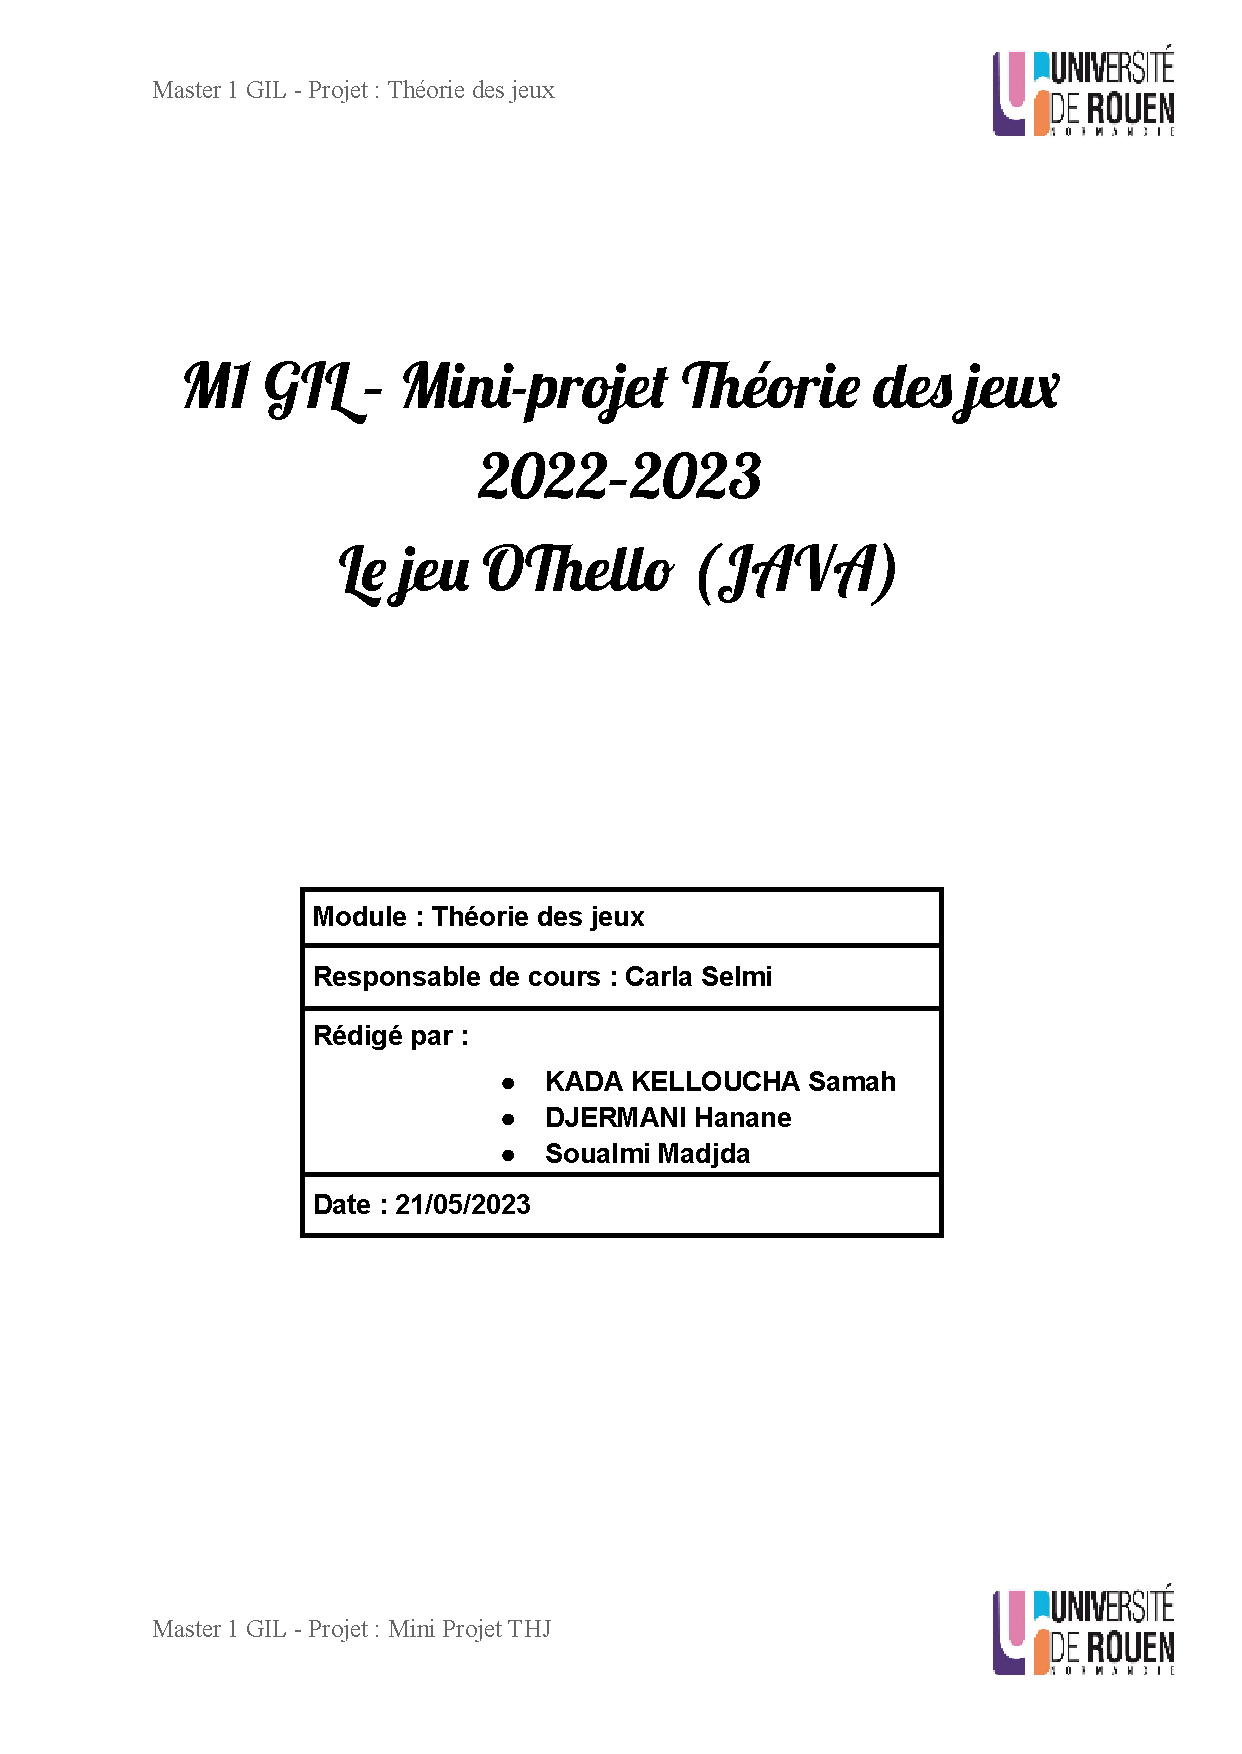
\includepdf{page.pdf}
	
	\newpage
	\tableofcontents
	\newpage
	\listoffigures
	\newpage
	\printglossary[title={Liste des Abbréviations}] %Generate List of Abbreviations
	\newpage
	%--------------------------Début de rapport ----------------------------
	\section{Introduction}

Jeu Othello, également connu sous le nom de Reversi, a été inventé au Japon en 1883. Il a été créé par un homme nommé Goro Hasegawa, qui l'a appelé Sekai no Hate Made (jusqu'aux confins du monde). Le jeu a été introduit aux États-Unis en 1975 et est rapidement devenu populaire dans le monde entier.

Le jeu se joue sur un plateau de 8x8 cases avec des pièces noires et blanches. L'objectif du jeu est d'avoir plus de pièces de votre couleur que votre adversaire à la fin de la partie. Les pièces sont capturées en les encadrant entre deux pièces de la couleur opposée, ce qui les retourne pour devenir de votre couleur.
\begin{figure}[H]
	\centering
	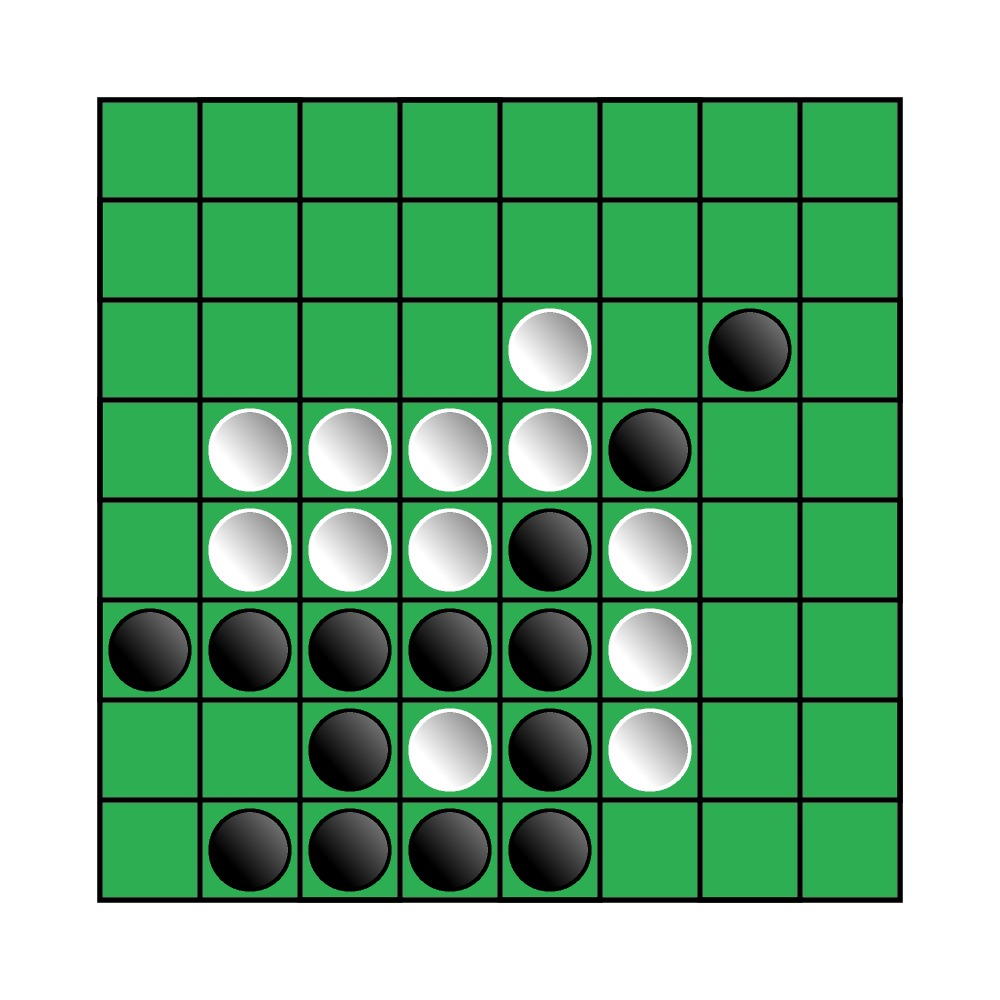
\includegraphics[scale=0.4]{img/othello}
	\caption{Le jeu Othello}
	\label{othello figure}
\end{figure}
\newpage
	\section{Travail demandé}	
Notre travail consiste à développer le jeu OTHELLO en utilisant différentes stratégies algorithmiques implémentées en Java.\\ Pour cela, nous allons programmer les algorithmes classiques de stratégies de jeu tels que \textbf{Min-Max}, \textbf{Alpha-Beta}, \textbf{A*}, \textbf{NégaAlphaBeta }et \textbf{SSS*}.\\ Pour une utilisation efficace de ces algorithmes, il est important de mener une analyse correcte du jeu.
\subsection{Les règles de jeu Othello}
 Les règles du jeu Othello, également appelé Reversi, sont les suivantes :\\
\begin{itemize}

	
	\item	Le jeu est joué sur un plateau de 8x8 cases.
	\item	Chaque joueur a un certain nombre de pions de sa couleur. Au début du jeu, deux pions noirs et deux pions blancs sont placés dans les cases centrales du plateau.
	\item Les joueurs jouent chacun leur tour. Le joueur avec les pions noirs commence la partie.
		\item Un coup consiste à placer un pion de sa propre couleur sur une case vide du plateau.
		\item Pour que le coup soit valide, le joueur doit placer son pion de manière à ce qu'il encercle un ou plusieurs pions adverses entre le pion placé et un autre pion de sa couleur déjà présent sur le plateau.
 	\item	Les pions encerclés sont alors retournés et deviennent de la couleur du joueur qui vient de jouer.
	\item	Si un joueur ne peut pas jouer, il passe son tour. Si les deux joueurs passent leur tour consécutivement, la partie se termine.
		\item Le jeu se termine lorsque toutes les cases sont occupées ou qu'aucun des deux joueurs ne peut jouer.
	\item	Le joueur qui a le plus de pions de sa couleur sur le plateau à la fin de la partie est déclaré vainqueur.
\end{itemize}
\subsection{Les Algorithmes demandés}
	    \paragraph{Min-Max [\ref{Algorithme MINIMAX}] :} Cet algorithme est une technique de recherche de l'arbre de jeu pour les jeux à deux joueurs. Il consiste à maximiser le gain possible du joueur en minimisant le gain possible de son adversaire. Pour chaque coup possible, il explore tous les coups suivants possibles et évalue le score obtenu pour le joueur en question. Ensuite, il choisit le coup qui maximise le score pour le joueur .
	    
	    
	    
	    \begin{figure}[H]
	    	\centering
	    	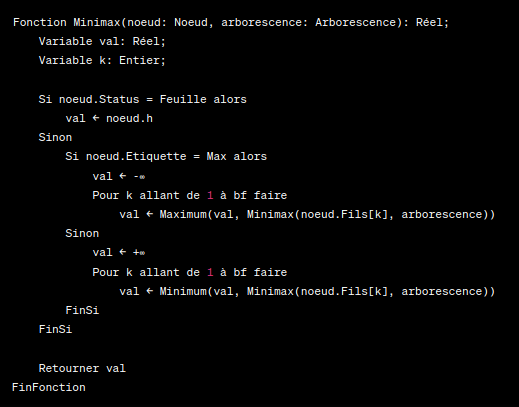
\includegraphics[scale=0.55]{img/minimax}
	    	\caption{Algorithme MINIMAX }
	    	\label{Algorithme MINIMAX}
	    \end{figure}
	\paragraph{NégaMax[\ref{Algorithme NégaMINIMAX}]:}L'algorithme Négamax est une variante de l'algorithme Minimax utilisé pour la recherche de coups optimaux dans les jeux à deux joueurs avec information parfaite, tels que les échecs, les dames et Othello.
	
	 \begin{figure}[H]
		\centering
		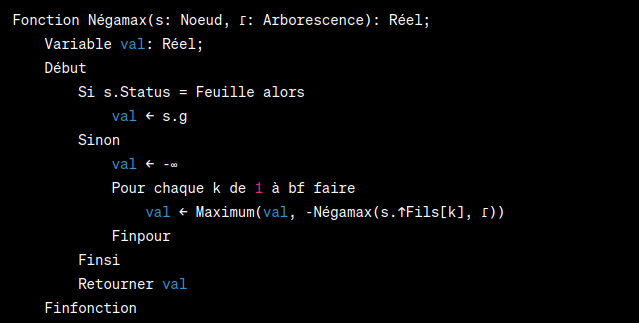
\includegraphics[scale=0.55]{img/negamax.png}
		\caption{Algorithme NÉGAMAX }
		\label{Algorithme NégaMINIMAX}
	\end{figure}
	
	
	
	
	\paragraph{Alpha-Beta [\ref{Algorithme ALPHABETA}] :} C'est une amélioration de l'algorithme Min-Max qui permet de réduire considérablement le nombre de nœuds évalués. Au lieu d'explorer tous les nœuds, l'algorithme Alpha-Beta utilise une technique de coupure pour éviter d'explorer des branches qui ne contribuent pas au résultat final. L'algorithme utilise deux valeurs, alpha et beta, pour suivre les valeurs minimales et maximales possibles.
	
	   
	\begin{figure}[H]
		\centering
		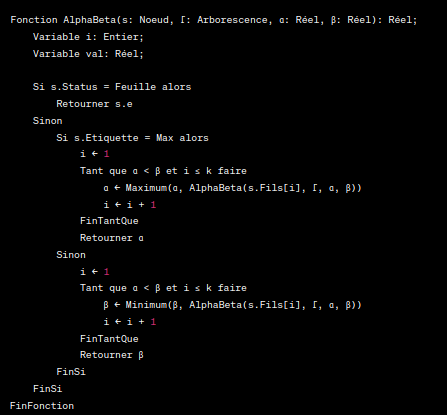
\includegraphics[scale=0.7]{img/alphabeta}
		\caption{Algorithme ALPHABETA }
		\label{Algorithme ALPHABETA}
	\end{figure}
	
	
		
\paragraph{	NégaAlphaBeta [\ref{Algorithme NégaAlphaBeta}]: }C'est une variation de l'algorithme Alpha-Beta qui est souvent utilisée pour les jeux à somme nulle comme l'othello. Il est similaire à l'algorithme Alpha-Beta, mais utilise une valeur de score négative pour le joueur adverse.
	
	
		   
	\begin{figure}[H]
		\centering
		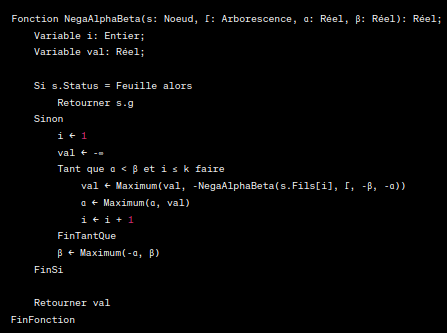
\includegraphics[scale=0.7]{img/negaalphabeta}
		\caption{Algorithme NégaAlphaBeta }
		\label{Algorithme NégaAlphaBeta}
	\end{figure}
	
	\paragraph{SSS* [\ref{Algorithme SSS*}] :} C'est une amélioration de l'algorithme A* qui utilise une liste ouverte de nœuds pour stocker les nœuds qui doivent encore être évalués. Contrairement à l'algorithme A*, qui utilise une file de priorité, SSS* utilise une liste liée. Cela permet de réduire le temps de calcul en évitant les opérations de tri nécessaires pour maintenir l'ordre de priorité dans une file de priorité.
	
		\begin{figure}[H]
		\centering
		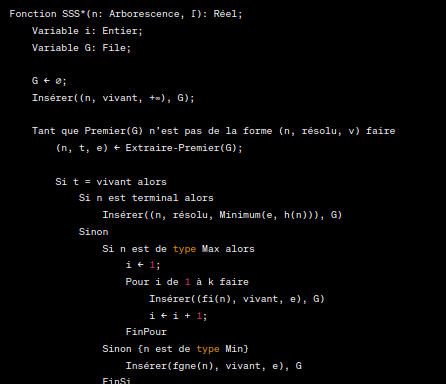
\includegraphics[scale=0.7]{img/sss1}
	\end{figure}
		\begin{figure}[H]
		\centering
		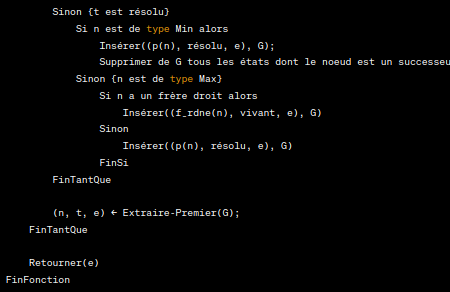
\includegraphics[scale=0.7]{img/sss2}
		\caption{Algorithme SSS* }
		\label{Algorithme SSS*}
	\end{figure}
	
\paragraph{	A* :} C'est un algorithme de recherche de chemin qui peut être utilisé pour trouver le chemin optimal entre deux points dans un graphe. Il utilise une fonction heuristique pour estimer le coût du chemin restant à partir du nœud actuel. L'algorithme explore les nœuds en fonction de leur coût total, qui est la somme du coût actuel et du coût heuristique estimé.

	\begin{figure}[H]
	\centering
	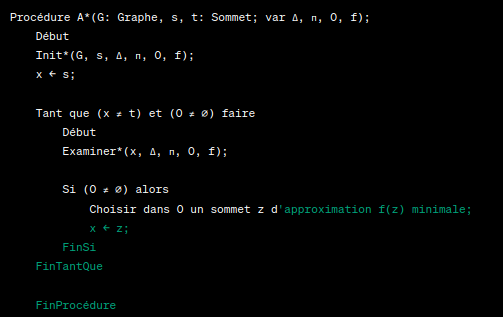
\includegraphics[scale=0.7]{img/A}
	\caption{Algorithme A* }
	\label{Algorithme A*}
\end{figure}



	


\section{Document technique}
	
		\begin{figure}[H]
		\centering
		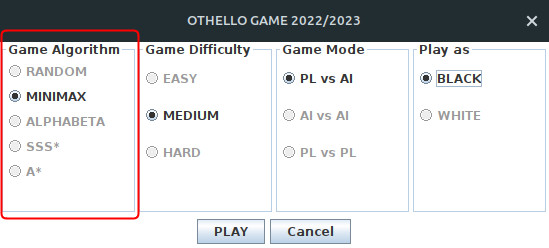
\includegraphics[scale=0.7]{img/othello_startAlgo.jpg}
		\caption{Choix d'algorithme }
		\label{Algo}
	\end{figure}

	\begin{figure}[H]
	\centering
	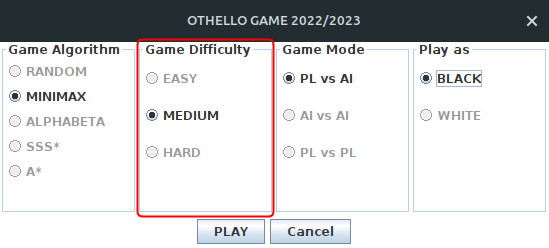
\includegraphics[scale=0.7]{img/othello_startNiveau.jpg}
	\caption{Choix de niveau }
	\label{niveau}
\end{figure}

	\begin{figure}[H]
	\centering
	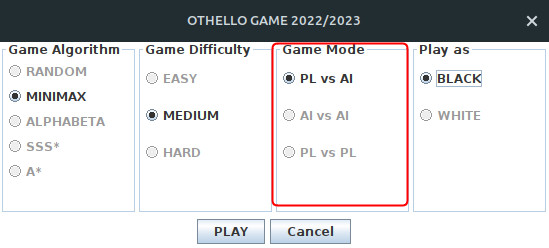
\includegraphics[scale=0.7]{img/othello_startMode.jpg}
	\caption{Choix de mode }
	\label{mode}
\end{figure}

	\begin{figure}[H]
	\centering
	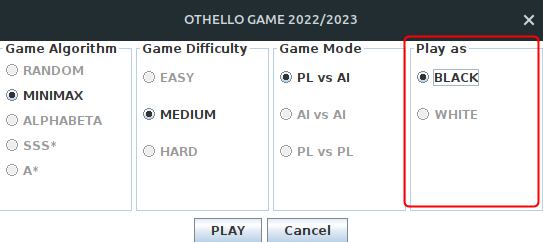
\includegraphics[scale=0.7]{img/othelloStartJoueur.png}
	\caption{Choix de type }
	\label{joueur}
\end{figure}
	
	
	
	
	
	
	
	
	
	
	
	
	
	
	
	
	
	
	
	
	
	
	
	
	
	
	
	
	%---------------------------------Fin de rapport---------------------------
	\section{Conclusion}
En conclusion, notre projet a consisté à réaliser le jeu Othello en Java en utilisant différents algorithmes de stratégies de jeu tels que MinMax, AlphaBeta, NegAlphaBeta, SSS* et A* malheureusement on à réussi à implémenté que les 4 premiers . Nous avons implémenté les règles du jeu et avons offert la possibilité aux joueurs de choisir leur niveau de difficulté ainsi que leur mode de jeu \textbf{(joueur contre joueur, joueur contre ordinateur, ordinateur contre ordinateur)}. Pour être efficaces, nous avons basé l'utilisation de ces algorithmes sur une analyse correcte du jeu. Ce projet nous a permis de renforcer nos compétences en programmation orientée objet ainsi que notre compréhension de l'utilisation des algorithmes pour la résolution de problèmes.
\end{document}